Since the methodology used has a bearing on the success of the project in hands. It is of high importance to choose which
practises should be adopted to effectively move forward. By means of this, investigation under which arsenal were to use is
counseled. After a lot of digging, it was decided that the number of different practises should not be to vast, otherwise it 
would be a burden to put them to work together seamlessly. 

Having a research methodology is full of advantages like: helping \textbf{plan},\textbf{structure} and \textbf{conduct} 
the research in a way which is structured and objective. 

Research methodologies can largely be categorized into \textbf{quantitative},\textbf{qualitative} and \textbf{mixed}. 
\textbf{Quantitative} focus on gathering numerical data and performing statistical analysis to draw conclusions. \textbf{Qualitative} 
on the other hand, is more suited to specify detailed insights such as behavior,motivations and experiences, which means that is more 
theoretical while the \textbf{quantitative} is more empirical. Finally, there is also the concept of \textbf{both} which stands for having 
both \textbf{quantitative} and \textbf{qualitative}.

During this thesis, in terms of research methodologies, there will only be space for two practises:  \textbf{DSR(Design Science Research)}, 
which in terms of nature of findings is hybrid, thereby categorized as a \textbf{both} approach like mentioned in the last paragraph and 
\textbf{SWOT} which is more \textbf{qualitative}. The first one is more complete and more suited for the projects while the second will 
be used more to drive the conclusions of the project to further analysis of it's pros and cons of usage of the project in cause. With 
all of these settled, lets move to deeper thoughts about each.

%
%
%    DSR
%
%
\subsection{Design Science Research (DSR)}
As an important gadget for the project, \textbf{DSR}  was the embraced tool. Considering it's traits, resembling extreme focus
on solving real problems, it represents indeed a powerful tool for going on with this thesis. Some people gain knowledge through
reading while other's achieve so by earring,practising or even speaking with other's. It's a serious challenge understand how a 
team will work best but,due to the nature of the team, \textbf{DSR} proved to be the best choice for it's phenomenal practise and 
rebuild model. In a distinct set of terms, this methodology is notably better for individuals which praise more the practical way of
things and by it's landing into the creation of artifacts for solving the current landscape of problems, creating this way solutions
and still gaining theoretic knowledge, it does outpace other methodologies making it better for the expected aspiration of 
this project \cite{dsr-book}.

\subsubsection{Goals of DSR}
For the verbal reference of the \textbf{DSR} goals, there is a colossal number of concepts that could be spotted as 
one. The gross of it, outcomes from the requirement of appeasing certain fields such as information systems,
engineering and others. This project is within the information systems realm, which means that these values are more than fit 
for the project and thereby qualified to be mentioned here. By means of this, the most captious goals will be pronounced here.

At the heart, \textbf{solving practical problems} is one of those goals. This is reached by the design and creation of such 
research artifacts that are implemented into practise, where those are seen as the form of models,frameworks,methods,processes,systems 
and even tools. With accordance to this means, practical problems are solved and theoretical knowledge comes as an extension.

Besides that, there is also the goal of \textbf{creating innovative artifacts}. It's presence is requested when it comes to push the
horizon of existing knowledge and capabilities. As Innovation takes precedence in any kind of project, it could not be different when 
it comes to the realization of this research, standing as a must for the \textbf{DSR}.

Tertiary to this, surges the \textbf{contributing to Scientific Knowledge}. Which is conventional, if further thinking is done through 
the definition and name of the methodology. Knowledge occurs by extension when depared with the solving resolve. Thus, the more knowledge
extended bigger the contribution and new perspectives and ideas may flow, creating an avalanche of future projects, instigating development
and furthermore improving sectors.

Onward to the next objective, there can be \textbf{Evaluation and Validation}, since the evaluation itself is a pillar for the loop
created within the \textbf{DSR} realm and so it is validation but, altought valid, it does not mean that it should be final. On this 
assumptions, rigid considerations must be accommodated, however, solutions keep maturing which explains the continuous satisfaction 
of this precise objective therefore nothing remains fully complete, which is expected from the point view of innovation.

Another objective important to consider is \textbf{Balancing Rigor and Relevance}, where it stands glamorously within \textbf{DSR} to 
make sure that nothing becomes to much theoretical until the point there is no practical implementation. This is a risk in the 
research world, where by applying to much importance to the theory category, the project start loosing color into it's true serving 
purpose. With this in aim, exists there the importance of instituting a balance between the two dimensions, emphasing both the theoretical 
inception but also the practical. This becomes the best approach, since the practical determines the verocity of the empirical sphere.

Lastly, there is the existence of another aspiration, denoted by \textbf{Generalizability of Solutions}. It's priority resides within the 
sphere of making sure that, knowledge produced within the project can be adopted into broader contexts, from a deck of various industries
or scenarios. This bears a huge relevance, because by having countless scenarios of usage,new use cases are produced, thereby relevance of 
the knowledge becomes enormous and so it's contribution for the research world, which affects the world by extension,purposionally to the desire of the 
research itself.

\subsubsection{The DSR Process}
\begin{figure}[H]
    \centering
    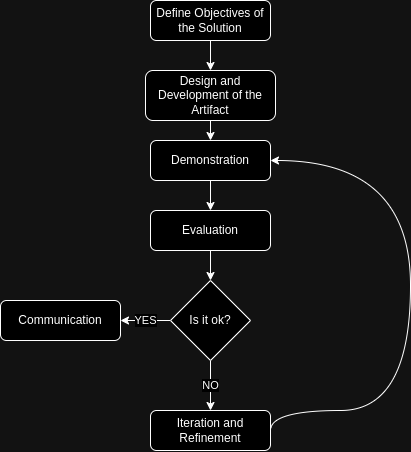
\includegraphics[width=0.5\textwidth]{assets/tools/dsr/DSR.drawio.png} % Change this to your image file
    \caption{DSR Life-cycle}
    \label{fig:sample-image} 
\end{figure}
Entering into the process of the \textbf{DSR} realm, there must be an understanding that this is a structured and iterative methodology, 
focused on construction,evaluation and improvement of \textbf{artifacts}. The process is extensive, but it covers all the steps necessary 
from problem identification to evaluation. Since it works around incrementation, this process is within a loop processing always new forms 
of solutions and knowledge, since it produces both \cite{dsr-book}.

\textbf{Problem Identification and Motivation} refers to the first step. Here, there is a preoccupation into picturing a real-world 
problem which seeks solution. To glean such information, various perspectives must be attended such as the current state,context and 
impact on the project under scrutiny. The spotted problem should be doted of meaning and with a given degree of relevance. The objective 
here is to gain power to articulate the problem clearly and make sure the team has the motivation for solve it. A good example to 
achieve this is in \textbf{healthcare, where there could be observed a problem with inefficiencies in patient management}.

As a second step, there is \textbf{Define Objectives of the Solution}. After problem identification, it is of huge gravity to think 
in a given set of objectives for the future solution. The objectives could be qualitative or quantitative, even thought the quantitative
are better, establishing them in the beginning is hard. Sometimes it is not possible and there are also situations where requirements 
already give them away. The objective in this step is to set expected outcomes and conduct obligations for the artifact that will be 
forged. An example for this would be setting an objective, \textbf{creating a system that should be capable of reach 50 request per second. 
But it could be a more simpler thing like giving good data for decision making in a healthcare facility}.

\textbf{Design and Development of the Artifact} surges as the third step. When landed in this step, there is work to develop 
the \textbf{artifact} (model,method,system or framework) that will be managed to meet the objectives created on the second step. With 
the problem and objectives on hand, the team must create,conceptualize and refine it's artifact to better meet the expectations. In another 
words, the objective is create a artifact that addresses these problems. \textbf{Developing a prototype of a healthcare data management 
system} can be a good example of what is expected in this phase.

Moving to the forth step \textbf{Demonstration}, here the \textbf{artifact} is assigned to work, by either creating a simulation or 
simply putting it in a real world system to check if it does meet the expectations. This stage is critical, because it serves as 
proof of concept to inquiry if it has utility or not. Regardless of the result, knowledge is generated and the \textbf{artifact} has 
room for growth because of the feedback created in this phase. The objective is to demonstrate if the problem can be solved or not with this 
implementation by a practical setting. One example of this would be the \textbf{deployment of a healthcare management system}.

\textbf{Evaluation} on another hand, corresponds to the fifth step, where the evaluation of the \textbf{artifact} takes place. In this phase,
the product is evaluated. Rigor,effectiveness,efficiency and overall impact are considered, taking into consideration the problem and that 
the evaluation method may defer relatively to the nature of the given product. This step has the objective of measure if the 
\textbf{artifact} solves the problem and meets the objectives settled in the earlier stages. As an example, the 
\textbf{evaluation of the performance by tracking the key metrics} can be considered.

At the realm of the sixth step, \textbf{Iteration and Refinement} is the step right after the evaluation. This is because, based 
on the observations, there may be areas where the \textbf{artifact} still lacks which compel for improvement. With this in mind, iteration 
is done and evaluation and demonstration occur multiple times until there starts to have insignificant improvements. As an objective, in 
this phase, there is the max refinement possible of the \textbf{artifact} recurring to iteration. To illustrate this, there is the 
possibility of image a case where \textbf{after testing, the system might be updated to include additional data fields or enhanced user 
interface features to improve usability}.

Finally, in the sept and last step there is the \textbf{Communication} phase. Within this, the research findings are shared, artifact 
design and theoretical contributions are released and the form it takes are \textbf{academic papers},\textbf{presentations} and 
\textbf{reports to stakeholders}. Deconstructing this, here there is the documentation and dissemination of the findings, including both 
practical and theoretical contributions. As an example, there is the \textbf{Publishment of a paper describing some development in healthcare 
made by a given research}.

\subsubsection{Usage during this project}

The usage of this methodology will be more comprehensive during the second use case. This is because the first one is more theoretical 
and the second is more practical. Since this approach goes around creating knowledge through a practical multiple loop iteration, it 
does require that the project is dotted of such.

With this in mind and better discussed further, firstly, within this work there is a definition of objectives for this solution. Secondly, 
there is the design and development of the artifact, which is a blockchain network. Thirdly, this network passes by a demonstration to 
effectively see how it behaves. Forthly, evaluations around the solution are made, and in case the solution is already good enough, 
communication is made; otherwise, there is once again a process of iteration and refinement that starts once again in the demonstration, 
creating this way an infinite loop until the solution satisfies the project needs.

%
%
%    SWOT ANALYSIS
%
%
\subsection{SWOT analysis}
\textbf{SWOT analysis} is a strategic planning tool which is often related to business. This is because it is a simple and yet powerful 
overviewer, that empowers organizations to set a plan for that precise moment. The acronymom \textbf{SWOT}, stands in English for 
\textbf{Strengths}, \textbf{Weaknesses}, \textbf{Opportunities} and \textbf{Threats}, which represent the key factors that influence 
the organizations success or failure. If done multiple times and by several people, it can gain multiple new perspectives that help as a 
decision factor because it can probably give a deeper understanding of the company competitive position, identifying potential areas for 
growth and also empower the staff to think better in strategies to address their challenges.
The purpose is to provide a well structured framework for decision making, which accesses internal factors like strengths and weaknesses 
and also external factors like opportunities and threats.
Despite it's current usage being more directed to business, it also helps in other kind of projects such as personal career planning and 
even research. In this project there's the intention to use it. This is because the use cases are complex, having a tool like this can 
help others understand the current situation, can help the stakeholders of the research to work according to the books and it can give a 
hint to those interested on the project to discover if it is doing well or not \cite{swot}.  

\subsubsection{Internal Factors: Strengths and Weaknesses}
Representing the upper part of the \textbf{SWOT} standard visualization, there is the internal factors 
\textbf{Strengths} and \textbf{Weaknesses}. This is what influences the most, the ability to the achievement of the 
organization objectives. Understanding both strengths and weaknesses is crucial as a building block for enhancing existing 
capabilities and check out areas where the organization usually outperforms or the opposite. To put in other terms, the organization 
has the capability for control and actively manage this two, in a way where the focus is to improve the decisions to do acomplish such.There 
are not always deterministic into that direction but deep dive into each will make this even more clear:

\paragraph{A. Strengths}\mbox{}\\
\textbf{Strengths} are the internal contributions, so that the organization has a certain number of attributes,resources and capabilities 
for enterprise level competitive advantage. These are the areas or aspects where the company can outperform others, that can be used to 
collect opportunities and even defend against possible threats. Identifying strengths is something very valuable for organizations, because 
it helps in focusing on the best attributes of the organization, thereby fixing their market position. As an example of Strengths, it 
could be something like: \textbf{Strong brand Reputation}, where a well established brand is widely recognized and trusted by 
consumers. \textbf{Skilled Workforce}, in cases where there is a qualified and experienced team who drive innovation and efficiency. 
\textbf{Proprietary Technology}, which are unique or patented technologies that provide a competitive edge in the 
market. \textbf{Operational Efficiency}, for processes and effective cost management that lead to higher 
profitability. \textbf{Customer Loyalty}, a loyal customer base that provides consistent revenue and positive word-of-mouth marketing 
and finally, more concretely for research, \textbf{Having more than enough resources}, which stands for having such resources that makes 
the research something more than feasible which usually is an huge challenge. By levering this strengths, an organization can maintain or 
even enhance it's market position, thereby maximize its competitive advantages in relation to others, improving by extension its overall 
economic performance.

\paragraph{B. Weaknesses}\mbox{}\\
\textbf{Weaknesses} are the core stone of the internal given limitations, for areas where the organization actually underperforms 
relatively to competitors which by extension can prevent the organization from achieving it's objectives, by representing a obstacle to 
the capitalization of the existing opportunities and even  by exposing the company to risks presented in external threats. \textbf{Weaknesses}, 
if spotted correctly, allow the organization to take measures for correctness and minimization of the impact that this unfortunate 
characteristics may pose in future iterations. Addressing this is essential for vulnerabilities mitigation, improve performance and 
prevent competitors from exploiting these causalities.
As an example, there is a lot of things that can be mentioned like: \textbf{Outdated Technology}, because by relying in older systems 
or tech can slow down processes,limit capabilities and even possibly increase costs for maintenance. \textbf{Limited Financial Resources}, 
where insufficient capital to invest can pose a problem to initiatives,R\&D and further expansion if desired. \textbf{Inefficient Processes}, 
in the idea of resource wasting and higher costs resulted from activities and delays in delivery. \textbf{Weak Brand Presence}, which 
represent a weakness in the essence of reduced market share and finally \textbf{High Employee Turnover}, where talent within the company 
is hard to maintain, thereby resulting in higher recruitment and training costs.

\paragraph{C. Both combined}\mbox{}\\
By understanding and analysing \textbf{Strengths} and \textbf{Weaknesses}, there is the possibility of creating a good synergy between 
both which can result in organizations positioning themselves to achieve their goals. \textbf{Strengths} help creating and sustaining 
competitive advantages and \textbf{Weaknesses} ensures that there are no barriers for further success. In other words, considering both 
interchangeably will imply future success, therefore it is very important to careful think in all of those and afterwards try to see it's 
relations.


\subsubsection{External Factors: Opportunities and Threats}
When it comes to external factors, there should be informed that those factors are the ones that the enterprise cannot control, since 
they don't own them and they are external to their direct manage. This means that despite the organization not being able to coordinate 
them, they can still take actions to make sure that those causalities don't affect them that much or that it don't affect them in any way. These aspects are \textbf{Opportunities} and \textbf{Threats} and they play a huge paper in the \textbf{SWOT analysis}. Putting in different terms, those are the existences that are based in outside situations that are beyond their control, such as market trends, macro-economic indicators, competition and others. \textbf{Opportunities} provide a path for growth, while \textbf{Threats} present a potential challenge that could negatively impact the company.
A deep dive into each factor will be done in this section:

\paragraph{A. Opportunities}\mbox{}\\
By identifying opportunities, organizations are doted of taking proactive steps toward expanding their market presence or even aggregating 
more into their competitive deck of cards. To achieve this, the organizations must attend to their external circumstances in order to 
effectively search over exploits that they can take into accordance to represent a new advantage. These, if used correctly, can help the 
organization grow, innovate and improve performance.
As an example, there is the following possible aspects: \textbf{Emerging Markets}, which stands for entering into a new geographic or 
demographic market, that offers potential for growth and expansion. \textbf{Technological Advancements}, that leverage new technologies 
that improve efficiency, number of product offerings or new innovative services.\textbf{Regulatory Changes}, related to new policies or 
regulatory shifts that if,taken into favor, can benefit substantially the organization in scope. \textbf{Shifts in Consumer Preferences}, 
that aims to answer to new consumer and trend behavior that can be targeted by a new product that may be on release and finally 
\textbf{Strategic Partnerships}, where forming alliances and collaborations with other companies can open new revenue streams.
By paying attention to opportunities, organizations can gain a competitive advantage, enter new markets and drive long-term growth.

\paragraph{B. Threats}\mbox{}\\
\textbf{Threats} on the other hand, are challenges or risks that could affect negatively the organization. Some of these are expected, but 
the worst ones are those that no one is expecting and because of this there must be a lot of thoughts about it, because a lot of this comes 
from disguised situations. Being able to spot such things, is a important skill when it comes to project maintainability and therefore it 
is specially important to pay attention to, because it can be the meaning of the project ceasing and catching them early can help to take 
preventive measures that could minimize or even remove the effects from it. Due to the external nature, the enterprise has low control over 
this kind of situations but being interested in such matters, can reduce significantly the downturns.
As an example, threats can be represent as \textbf{Increased Competition}, where the increase of offers of similar products can 
potentially remove some market share. \textbf{Macro-economic downturns}, where the economy slows down for some reason which results in 
less demand for the project. \textbf{Regulatory changes}, which can result in the enterprise suffering by politics that may be against it 
or that revoke previous given benefits. \textbf{Changing Consumer Preferences}, that happens when the consumer shifts it's interest in the 
current product and benefits the competitor leaving the organization behind and \textbf{Technological Disruptions} where the advances in 
technology actually removes the need that the enterprise was serving, therefore making the organization service/product obsolete.
In case well informed, organizations can adapt and overcome this challenges, by preparing defensive strategies that will mitigate 
risks,ensure business continuity and market share protection.

\subsection{Risk List}

In the following table, the risks that directly or indirectly influenced the development of this dissertation are listed. Depending 
on the identified risk, a mitigating action is proposed in order to minimize the impact of the risk. The scale for the Probability and 
Impact columns is measured from 1 to 5, where 1 corresponds to a very low risk and 5 to a very high risk.

\begin{longtable}{|c|p{2cm}|c|c|c|p{2cm}|c|} 
    
    \hline
     \textbf{Nº} & 
     \textbf{Description} & 
     \textbf{Probability(P)} & 
     \textbf{Impact(I)} & 
     \textbf{Seriety(P*I)} & 
     \textbf{Mitigation Action} & 
     \textbf{Verified}  
     \\ \hline
    \endfirsthead

    \hline
    \textbf{1} 
    & 
    Unreachable deadlines
    & 3 
    & 5 
    & 15 
    & Planning better the next events and gain experience from previous deliveries;
    & Yes 
    \\ \hline
    
    \textbf{2} 
    & 
    Requirements of the project change
    & 2 
    & 4 
    & 8 
    & Make frequent communication with stakeholder;Check well the limitations imposed by the project;
    & No
    \\ \hline
	
    \textbf{3} 
    & 
    Lack of Time
    & 4 
    & 5 
    & 20 
    & Implement only what is actually needed
    & Yes
    \\ \hline

     \textbf{4} 
    & 
    Resources
    & 4 
    & 5 
    & 20 
    & There are no mitigation measures
    & Yes
    \\ \hline

     \textbf{5} 
    & 
    Incorrect understanding of data
    & 2 
    & 5 
    & 10 
    & Spend more time analyzing the data; Make sure that the data is relevant for the object of study;
    & Yes
    \\ \hline
    \end{longtable}
    
    
    
    \begin{longtable}{|c|p{2cm}|c|c|c|p{2cm}|c|} 
        \hline
     \textbf{Nº} & 
     \textbf{Description} & 
     \textbf{Probability(P)} & 
     \textbf{Impact(I)} & 
     \textbf{Seriety(P*I)} & 
     \textbf{Mitigation Action} & 
     \textbf{Verified}  
     \\ \hline
    \endfirsthead
    \textbf{6} 
    & 
    Mistakes
    & 1 
    & 5 
    & 5 
    & Don't do tasks in automate mode; Focus more in the tasks;
    & Yes
    \\ \hline

    \textbf{6} 
    & 
    Security implications
    & 1 
    & 5 
    & 5 
    & Follow standards; Try to learn more as the time passes;
    & No
    \\ \hline

    \textbf{7} 
    & 
    Complexity of the project
    & 2 
    & 3 
    & 6 
    & Document Everything; Simplify everything;Join Communities;
    & Yes
    \\ \hline

    \textbf{8} 
    & 
    Unknown Errors
    & 2 
    & 4 
    & 8 
    & Join Communities;Arrange more debug mechanisms;
    & Yes
    \\ \hline

    \textbf{9} 
    & 
    Acceptance
    & 4 
    & 5 
    & 5 
    & Make the best solution possible;Make clear the need of the solution;
    & No
    \\ \hline

    \caption{Risk List: General} \label{tab:activity_schedule} 

\end{longtable}

\subsection{Relevant tools}

Before delving into the use cases and what were done in practical terms, there is a need to explain seamlessly which tools were 
used during the project. This is because, by explaining what was used, by extension, an assumption by the reader for the reason why 
certain things were inserted in the project is achieved. Some tools are related to blockchain, since that is the main subject under 
scrutiny along with the healthcare sector, but others, on the other hand, are extensions of a product that is strong by itself. Reasons 
for the usage of blockchain were already mentioned in the State of Art; thereby, there is no reason to go much deeper in this aspect, but 
returning to the other tools, they are needed for commodity purposes, and probable risks resulted by the usage of certain tools will be 
covered further in this thesis. Also, it is important to mention that the idea around this project is not to achieve excellence in 
decentralization or to simply use emergent technologies because they are trendy, but to try to solve the existing problems with the best set 
of tools that are proven to be the best in the current market and perhaps standardize the way private blockchains are designed to gain broad 
acceptance. Standardization helps with broad acceptance because this way implementations are not that fuzzy like they were before, 
contributing to ease in implementations and creating a common path between people that, in case of obstacles, there may be a current 
solution already because someone crossed the same path before. This is essential for a vast spread adoption, and thereby that's our 
contribution here.
There are 3 covered sections within the tools; the list is not at all complete, but there is an effort to cover the most important concepts 
of technologies that were used during the project. This will empower the reader with the correct view of what has been done so far.
There is a Microservices section in which the tools are a part of the other tools that will be covered. They retain an honored representation 
on this project because their usage is meant to empower administrators with capabilities such as resource management, easier setup of 
networks, decoupled services, scalability, and high availability.
Another important section is analytics; this is very important for any type of robust system, and its aim does not reside only in 
maintainability. It empowers the project with also mechanisms to detect bottlenecks, detect unexpected behavior, troubleshooting support, 
debug support, benchmarking, observability, measures to better resource management and more.

Finally, there is also the web development section, which is used in this project as the core to build extra services that may be required
for the normal function of the network. They work mostly for communication support, for ensuring security, and to help automate procedures 
during the results obtained in this research, but also for future usage while using this in a real environment.


\subsubsection{Blockchain}
This section will contain all necessary related or close related information about blockchain that is being used in this research. The 
aim in this section is to give a good fundamental overview about \textbf{Hyperledger Fabric}, the private blockchain technology that 
is used all over the investigation and also to give some hints about \textbf{IPFS}, which despite not categorized as a blockchain, has a 
lot of characteristics that resemble a blockchain thereby despite the section name, it still makes sense to put it here for the purely 
sake of relation between the concepts making it easier to digest. The first is considered a general purpose technology, 
which can be used with all kinds of data but having the capability of working with all kinds of data and at the same time be capable 
of dealing with all types in a effective way that's a completely different story and, because of this and also to respect to files, there 
was a need to think in a extension of the blockchain capabilities where \textbf{IPFS} can effectively play its rule. Altought intriguing, 
in this work there was not a measurement of performance regarding this technology and how it would behave in the private landscape, which 
means that atleast in this realm there are no tangible evidence of effectiveness on our side, which may result in the future measurements 
while working interchangeably with both the blockchain and this technology for storing files, exacly like describe in one of our future 
mentioned use cases.

\paragraph{3.5.1.1- Hyperledger Fabric}\mbox{}\\
\textbf{Fabric} is an open source permissioned distributed ledger platform designed for use in enterprise contexts, delivering a 
certain number of capabilities that are imperative in business scenarios. It is maintained by the \textbf{Linux Foundation}, and it presents
an architecture that is modular and also configurable. It supports smart contracts through general purpose programming languages 
like \textbf{Go}, is permissioned, has pluggable consensus protocols that range from existing default ones to custom, does not require 
a native cryptocurrency and offers one of the better performing platforms today of this kind for transaction processing and 
transaction confirmation latency \cite{hyperledger}.

This framework will be intensively used in the provided use cases. With this in mind, this section will be a solid coverage all over 
the main concepts of this framework.

Relatively to \textbf{Permissioned Networks}, this is a concept relative to a type of blockchain. Dissimilar to public blockchains 
such as \textbf{Bitcoin} and \textbf{Ethereum}, often called \textbf{permissionless} blockchains, these ones 
restrict access to a set of known participants, making them ideal for applications that require trust and control over the 
membership. Like mentioned before, \textbf{Hyperledger fabric} is one of these types, and so is \textbf{Corda}. Both 
platforms emphasize accountability without relying on a central authority, enabling organizations to construct custom 
and heterogeneous applications where there is a clear conscience of who can participate in the network \cite{permissioned-blockchains}. 
Usually, the usage of one restricts the usage of the other.However, there are also approaches where networks 
may want both \textbf{permissionless} and \textbf{permissioned}, referred to as \textbf{two-tier blockchain}, where both 
types are combined to allow both participation and validation, such as supply chain or cross-border financial 
transactions \cite{two-tier-permission-blockchains}. For the context of healthcare, \textbf{permissioned} is obviously 
more appealing, such that \textbf{operational efficiency} and \textbf{transaction security} when combined with restricted 
trust between participants is needed for \textbf{security} and data \textbf{privacy} \cite{permissioned-vs-permissionless-tradeoffs}.

Furthermore, there is also the modularity of \textbf{Hyperledger fabric} to be covered. It has 5 components: the \textbf{Peer}, 
\textbf{Orderer}, \textbf{Chaincode}, \textbf{Ledger}, \textbf{CA's (Central Authorities)}, and \textbf{client}.

\begin{figure}[H]
    \centering
    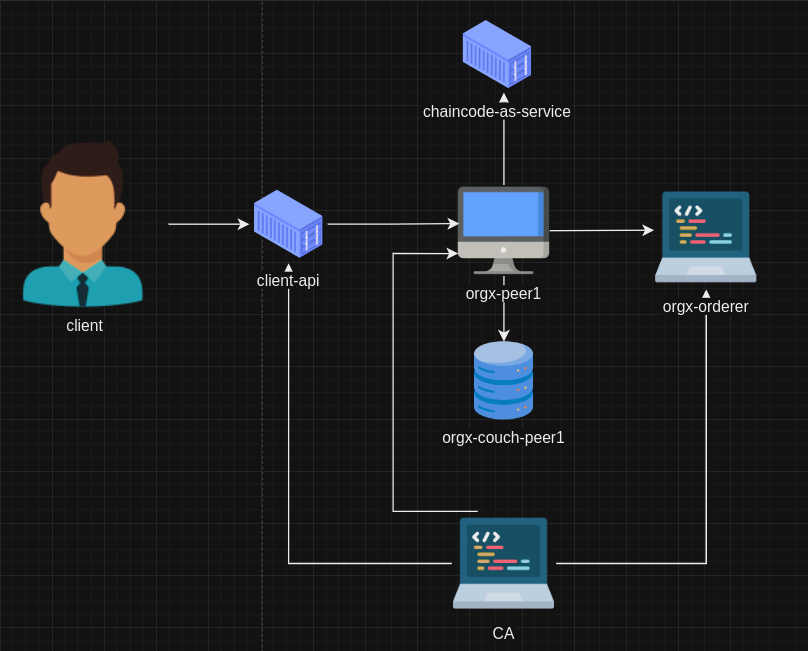
\includegraphics[width=0.5\textwidth]{assets/tools/hyperledger/hlf-minimal-setup.png} % Change this to your image file
    \caption{Major components Relationship}
    \label{fig:sample-image} 
\end{figure}

As an overview above, there is an image that illustrates not the communications but how components 
may relate with each other. Also, it should be noted that this is very far from representing a whole system, where usually 
multiple peers must endorse transactions and multiple orderers must order transactions and blocks. Putting in another terms, 
the representation here explained is just for the sake of understanding how individual components work with each other. With 
this in mind, each component's individual functions will be covered more ahead.

The \textbf{Peer} (orgx-peer1) in this representation is the middle point of everything. This is because it is the one that receives 
the transaction proposals and endorsements that come from other peers by previous request of a client. It also receives blocks 
from the \textbf{orderer}, and it is responsible for endorsement of transactions by using the \textbf{chaincode}, and furthermore, 
after validation through this \textbf{endorsements}, it is the one that receives a \text{block} containing valid transactions 
from the \text{orderer} (orgx-orderer), for then to include in it's \text{ledger} (orgx-couch-peer1). The \textbf{client}, on the other
hand, manifests in two ways: the client itself as an actor and the \textbf{client-api}, which turns out to be the application 
itself that is responsible for calling the \textbf{Peer}. The \textbf{chaincode} (chaincode-as-service) simply runs logic, which is 
what the \textbf{Peer} endorses, by running the application against the \textbf{ledger} (orgx-couch-peer1). In respect to the 
\textbf{ledger}, it is used as a mock to endorse transactions to see if the output is the same within the vast majority 
of peers.The \textbf{orderer} receives transactions and puts them inside of blocks, and after ordering these transactions and 
blocks, it delivers the blocks to the peers. Finally, the \textbf{CA}(certificate central authority) only gives cryptographic 
materials so that components can identify themselves within the network. It must be known as well that the chaincode-as-a-service 
has the option to create TLS connections with the peer. In this picture there is only one CA for purposes of simplicity on this 
explanation, because usually there can be a chain of CA's and in each level, for purposes of good practices, should have 2 CA's 
where one is for normal certificates and the other is for TLS. The difference between normal and TLS certificates is that 
one is for identification and the other is to secure the communications with encryption. Once again, in this representation only 
normal certificates are considered, but within the network there are both, which contribute to a secure 
environment. \cite{rfc5280}.Now that their relations were described, let's describe them in more deep terms for further explanation.

In what concerns the \textbf{peer}, this is a fundamental concept within the network since it is responsible 
for managing \textbf{ledgers}, \textbf{smart contracts}, \textbf{transaction proposals}, and \textbf{endorsements}. \textbf{Ledgers} and 
\textbf{Smart contracts} will be explained further, but a transaction proposal is a transaction that was signed by 
some entity that wants to be further endorsed by the peers for then to be included in the ledger if valid. \textbf{Endorsements}, on 
the other hand, are the process of a peer running the logic within the proposal against its ledger. Depending on the configuration of 
the channel and the number of peers that validated this proposal, this transaction will be included on the block 
or not (within the orderer side); therefore, it could be or not included in the ledger depending on its validity.

In the \textbf{Orderer} sphere, however, there is the responsibility of receiving endorsed transactions, which, 
depending on the number of signatures of the peers in it, could add the transaction to a block or reject it. In the case of the first,
after ordering the transactions and the given blocks, it returns to all the peers this given block. Block this that will be used 
for the peer to insert its operations against it's ledger, therefore ensuring that every single peer has the same view of the state 
because they are all running the same operations against the same state. To achieve this, the orderer uses what is called a 
\textbf{consensus protocol}. This protocol is a mechanism to reach agreement in the sequence of transactions, but that will 
be discussed further.

Another vital pillar for the network is the \textbf{Smart contracts}, more commonly called \textbf{Chaincode}. This is where all of the 
business logic runs, and it uses abstractions to communicate with the ledger. Usually, installation is required only once. However, it 
must be added per channel if that is the intention of the participants within that channel. This means that I can have the chaincode 
installed, but this chaincode could potentially not be allowed to be called because, for that, it must be proposed to be added and 
committed when a certain number of participants agree on its insertion. Besides that, there are 2 typologies for usage of 
chaincode: \textbf{normal chaincode installation}, which occurs per peer and the chaincode becomes more like a side 
container, and \textbf{chaincode as a service}, where the chaincode becomes a service and to install it there must be passed metadata 
for the connection management. The normal way is often used for questions of ease, and, along with it, there is the certainty that 
the chaincode that is being invoked is in fact the desired one, since it is literally a side container or side service of the peer, 
therefore also giving more isolation to it. The other way, however, depending on how it is deployed, it can be reused by 
multiple peers, which means that if an operator does not retain this service within its infrastructure, it may represent a 
risk since the endpoint could be the same and its application could be changed. Be mindful that, in case 
the \textbf{chaincode as a service} is adopted, depending on how it is implemented, it can be exposed to the common microservices 
vulnerabilities, and further actions should be taken to prevent these \cite{microservices-common-vulnerabilities}.

\textbf{Ledger}, on the other hand, is a normal database like \textbf{couchdb} \cite{couchdb}. This is the state that the 
\textbf{Peer} uses as a mock to run its business logic and get an output for later usage for the endorsement procedure. Transactions 
can be rejected by either violating some business logic or by presenting different outputs among the peers. As an example, let's suppose 
there are 3 peers. In the first situation, peer 1 rejects the transaction because the business logic says so. The other 2 peers, peer2 and 
peer3, respectively, accept the transaction. In the case of a majority policy, the state resulted in peer2 and peer3 being included 
in peer1 as well, simply because the majority wins. Also, let's consider the case where peer 1, peer 2 and peer 3 have different outputs, 
but the signatures were still reunited because the transaction was not rejected. What will happen is that when this transaction reaches the 
orderers, the orderers will reject its validity. This is because, despite passing the peer endorsement, the orderer endorsement will fail due 
to a lack of determinism between the three peers. Also, within the same database, there could be different slices of data for 
each \textbf{channel}. However, the concept of channel is something that should be delved deeper into more ahead.

Speaking about \textbf{CA's}(Certificate Central Authorities). This is a service that serves cryptographic material like private 
keys and x509 certificates, which within a \textbf{hyperledger fabric} network form a \textbf{MSP} (Membership Service Provider). \textbf{MSP}
is a mechanism designed for providing a way to offer identities that could be trusted and recognized by the rest of the 
network. To achieve this, there is the usage of this cryptographic material provided by the CA's where a key 
pair is offered. One of these pairs, the private key, is used to sign transactions, and the other, which is public, gets shared among 
the entities that will be communicating with the owner of the private, giving them a way to verify that this signature is actually 
valid. \textbf{Hyperledger} lets the operator either rely on existing public CA's, use their CA implementation, or simply use 
a \textbf{hybrid} methodology. The main difference between the public and their implementation is that it's implementation already 
comes with a given file structure to make the configurations easier and also the aggregation of more responsibility to the operator, but 
that's something that is not the concern here, thereby it should not be extended.

Relatively to the \textbf{client} within the hyperledger fabric components sphere, there is a close relation in
how it operates with the chaincode. Like chaincode, both can be implemented with a certain number of
high-level programming languages such as \textbf{Go}. Both use an interface, attributed to their set of tasks in aim.
In the case of the \textbf{chaincode}, its interfaces are related to making interactions with the ledger, but in the case
of the client, its abstractions are focused on making calls against the peer by giving metadata related to
the \textbf{channel} and methods to be targeted. Thus, it’s more formal name is \textbf{Fabric SDK}, where there is the
opportunity to use \textbf{Node.js}, \textbf{Java}, and \textbf{Go}. Giving the opportunity to perform various functions, such as
creating \textbf{channels}, submitting \textbf{transactions}, querying the \textbf{ledger}, and managing the \textbf{chaincode}. Within
the \textbf{SDK} ,there are various subpackages aimed at serving different purposes, like: \textbf{gateway}, for establishing
connections to the network and provide access to \textbf{channels} and \textbf{contracts}. \textbf{Network}, which represents
a channel that a client can interact with. \textbf{Contract}, conceded for iteration with a given smart contract
deployed in a \textbf{channel}, used for submitting and evaluating transactions, and finally Wallet, responsible for
managing user identities and credentials for connecting to the \textbf{fabric network}. Further details should be
seeked within the proper documentation of \textbf{hyperledger fabric}.

Apart from what has been covered so far, there is the concept of \textbf{channel}. This concept is very important since it is the existing 
mechanism that allows you to aggregate a certain number of components, thereby creating a linkage between them and a precise section for 
them to exchange information. Within the documentation of \textbf{Hyperledger Fabric}, there is the reference to channel 
as a \textbf{group of friends}. This is because, exactly like a channel, you have multiple groups of friends on your social media and 
their members are different depending on the task or the theme to be discussed within that group. Also, within those groups there is an 
exchange of information that is private and it's not shared with other group members, which is essentially the same thing as a channel. In 
a channel, you aggregate a certain number of components that could be part of multiple different organizations depending on what you want 
to be sharing within that channel, and also within this channel, there is the option to create a \textbf{private collection}. Despite the 
theme being the same, there are participants that may want to discuss information regarding this discussion within the group but 
just with a set of participants, especially like it would be with the private collection. Though the difference with a friend group is 
the nature of blockchain. This means that with a private collection, there is the option of creating a subset within the channel, making 
others able to see that you are communicating with each other but not what they are exchanging. In other terms, a given organization can 
be in multiple channels, with multiple different individuals in each, and it can also create multiple private conversations regarding 
the same theme, but just with a subset of participants in the same channel and exclusively of that precise channel. As an example, 
let's think of an organization that has the idea of creating a group of medicament's suppliers and other group of medical clinical 
reports. Obviously, in these examples, there will not be common participants because their nature is different. The organization may 
discuss within that group that it needs medicaments for X. Supposing they want to buy the cheapest one, they will request it from the 
enterprise Y. This enterprise, although offering it more cheaply, may not have the quantity to satisfy this need, making this organization 
forced to go to supplier Z to satisfy the rest of the demand. Maybe, for the benefit of this organization, prices of the product 
should not be known by the participants within this channel, which means that at least the monetary transactions within this channel 
should be done in private collections. However, the transactions of products could be done publicly, therefore making it easier for all 
of the participants to have the information publicly available that this organization is supplying itself from these two organizations, 
making others in the obligation of trying to bargain to also benefit from this channel. Also, the same applies to the clinical registry, 
even if it has a different logic or idea. There may be information that can be publicly exchanged between doctors, but there may also 
be communication that should only be sent within a more restricted set of individuals within that consortium. With channels and private 
collections, hyperledger obtains data confidentiality,selective data sharing and regulatory compliance \cite{private-collections}. 

\textbf{Endorsement Policies} are another big dinosaur in the room when speaking about \textbf{hyperledger fabric}. These are the 
rules under which the transactions will need to apply, making the transactions valid in case they succeed and invalid in case they 
fail to do so. In other terms, these are the policies that define which peers must sign (endorse) a transaction before it can be valid 
and aggregated to a block by an orderer. It specifies how many and which organizations must approve the transaction before it can be 
inserted into the ledger.

Piercing to the real use cases realm, there are several occurrences of hyperledger appliances. The sectors affected by this remarkable 
technology were: \textbf{Financial},\textbf{Healthcare},\textbf{Supply chain management},\textbf{Goverment and Public Sector} and 
\textbf{Insurance}. Within the \textbf{Financial}, various banking consortiums were created for processing cross-border payments, managing 
the financial chain, and enabling transparent asset transfers \cite{finances-use-case}. In the \textbf{Healthcare} there are also a 
lot of occurrences of it's usage for managing electronic health records (EHR's), which is possible due to the channels and private 
collection capabilities, allowing sharing of patient data between healthcare providers \cite{healthcare-use-case}. In the 
\textbf{Supply chain management}, there are multiple occurrences for the usage of hyperledger fabric for tracking goods. By using 
this, enterprises were dotted of track food products from the farm until the shelf, reducing the time required to trace the origin of 
food products in the event of contamination while still offering privacy for sensitive business data using private collections 
\cite{supply-chain-use-case}. Also, when it comes to \textbf{Government and Public Sector}, it is well known that there are already 
present in the market implementations for the usage of such technology for managing digital identities, land registries, and transparent 
voting systems \cite{public-sector-use-case}. Finally, there is the usage for \textbf{Insurance}, where there are retained implementations 
that are meant to help claiming processing and reduce fraud. Thus, by levering this, the \textbf{Insurance} can collaborate in a 
shared ledger to verify these claims and manage shared data, reducing duplicated and fraudulent claims \cite{insurance-use-case}.

\paragraph{3.5.1.2- Ipfs}\mbox{}\\
When it comes to \textbf{IPFS}, it must be known that this does not represent a blockchain, though its concepts derive from a 
P2P perspective, which means there are relations between the two. It is a modular suite of protocols for organizing and transferring 
data \cite{ipfs}.

More concretely,\textbf{IPFS} is a tool that stands for Interplanetary File System, where it refers to an implementation that was meant 
to become the file system of the future.

This solution can be interplanetary, because when the first request of a file in the network occurs, it may endure a lot of time, but 
after getting it, the file will be retrieved faster because it will be stored in cache in the most nearby peer. Thereby, if you plan to 
travel to another planet, it can be possible to share files in this network, which, depending on the range, may also include other planet 
files, but this has countless ways to occur. Or either by one of the peers from another planet changing its location to a location that is 
reached by our network or simply because the connection between those 2 planets is feasible. However, in order for this to work, there is 
still work related to making sure that the files are pinned; otherwise, they will get deleted later by garbage collection. This ensures 
that we do not have files permanently. If they are not that relevant, with time, they will simply disappear \cite{ipfs-overview}. 

\subsubsection{Microservices}
Within this section, there is information about the major high level technologies that were used in this precise research that are related 
to \textbf{microservices}. One of those technologies is almost a obligation for the current landscape of technology, there is one which 
is a upgrade, one that is necessary in certain concrete situations and there is also a extension but all of them are valid. The one that 
is almost a obligation is docker, because currently in the tech landscape it is used in almost every system because of its isolation 
therefore faster for development in big teams. The upgrade is the kubernetes, which manages this \textbf{docker} images like they are 
resources ,making it complex in a certain way but also easier to manage in another after learning it. The necessary in certain concrete 
situations, in another hand is \textbf{MetalLB}, because it is meant to on premise implementations, which means that it is more suited 
for own infrastructure implementations which is a big help when it comes to healthcare due to their resistance into moving to 
the cloud. Finally the extension is \textbf{Istio}, because it is used to have more control over the network and its communications, but 
its usage its not mandatory, thereby in this project despite tested it is not used in any implementation.
After \textbf{Hyperledger}, this are the technologies that more represent how some implementations communicate, therefore is good to 
present what they are and how they work, so the reader can understand the architectures that will be presented further. 

\paragraph{3.5.2.1- Kubernetes}\mbox{}

\textbf{Kubernetes} stands as a open-source platform designed for \textbf{automating the deployment},\textbf{scaling}, 
\textbf{management of containerized applications},\textbf{management of resources}, \textbf{management of secrets} and 
\textbf{management of configurations}. Originally developed by \textbf{Google}, \textbf{kubernetes} has become a standard for 
managing containers being a premise to build cloud-native applications. By taking leverage of this, developers can abstract the 
infrastructure and focus more into the application logic instead of hardware and other operations side tasks. With this in mind, 
\textbf{kubernetes} today is centered as the pilar for building any application, even if it is on-premise(within a organization 
own infrastructure), due to the fact that currectly every organization seeks a \textbf{microservices architecture} which obligates 
businesses to build their own kubernetes clusters. This is because, microservices itself offers a lot of advantages for their business 
such as \textbf{high-availability} because of deployments, \textbf{better resource management} and \textbf{resilience} which are crucial 
for any organization that wishes to remain competitive \cite{kubernetes}. 

\paragraph{3.5.2.2- Docker}\mbox{}\\
\textbf{Docker}, on the other hand, is a technology that could be abstracted by the previously mentioned \textbf{Kubernetes} and is 
said to be a tool to build applications in a different paradigm than before. To contextualize, in the past it was something normal to 
install dependencies directly in your local machine, which created some burden since you may have had different projects with different 
dependencies versions. Also, the application would mess with the local machine configurations because it was directly using it's resources, 
having more probability of making adjustments that would compromise other projects by having different configurations. By acknowledging these 
limitations, Docker came to light because it was conceded to automate deployment, scaling, and management of these referenced applications 
using a new concept called \textbf{containerization} \cite{docker}.

\paragraph{3.5.2.3-MetalLB}\mbox{}\\
\textbf{On-premise cluster} is an advanced concept related to setting a network of computers within your own infrastructure. In the case 
of this project, the reference to this is related to a network composed of \textbf{kubernetes} nodes. Because of this, it is imperative 
to mention \textbf{MetalLB}, which is a \textbf{load balancer} conceded just for \textbf{on premise Kubernetes clusters} \cite{lb}.

When it comes to \textbf{kubernetes}, usually the tendency is to relate it to the cloud. However, as the time progresses, components 
become more powerful and cheaper, and more and more, the consideration of moving to the cloud or not becomes more a question of cost and 
responsibility. This is because, though the power of components is becoming stronger, the complexity of hardware is sometimes increased, 
making organizations choose between being themselves responsible for the maintainability of the infrastructure or simply giving it away to 
those that are more specialized in the subject, which may or may not reduce costs for them because not only do they have the common 
infrastructure costs but also the burden of finding and maintaining qualified personnel for this type of job \cite{onpremice-cloud}.

\textbf{MetalLB} comes into play when it comes to those more audacious to have all the responsibility. As a strong \textbf{Load Balancer} 
for \textbf{on premise} networks, it stands in this project as a marvelous tool for achieving load balancing, which is a concept 
where the requests are distributed through multiple instances of the same application, balancing this way the load that each may have. Cloud 
distributors have their built-in support for such, while on-premise networks do not, which makes \textbf{MetalLB} a must for setting 
such capability in a non-cloud environment.

\paragraph{3.5.2.4- Istio}\mbox{}\\
In this thesis, \textbf{Istio} appears more like an extension and not concretely as something that was of extreme usage. However,
because it was used to determine in each measure is useful and also because it is very different from other concepts, explanations 
over what it is are required because, although not extensively used, it is mentioned in the thesis \cite{istio}.

\textbf{Microservices} is an architecture of exalted power. However, what comes with great power also requires great responsibility. Therefore, 
conducting the management of the communications between services is not a straightforward task. By virtue of such, the more 
the application expands, the more work there is around this matter, making \textbf{DevOps} teams struggle when it comes to make 
optimization and manage this within the application realm.

By means of this, \textbf{Istio} surges as alleviation of such. At the hand of its capabilities, it serves as a \textbf{service mesh}, which 
is nothing more than an abstraction created around the application for providing \textbf{Traffic Management}, \textbf{security}, 
\textbf{Load Balancing}, and \textbf{monitoring}.

As mentioned before, cloud-native architectures and microservices are becoming something permanent. Such that managing it is a challenge. Thus, 
using a \textbf{Service mesh} could potential be something meaningful because it works as an abstraction layer that handles the 
dynamic networking and communication between microservices. With this brief introduction in mind, thinking in the most important aspects 
for which this is needed is something intriguing. Firstly, \textbf{enhances microservice communication and networking} is one of the 
aspects for including istio. This is because, a service mesh provides service-centric networking, thereby oferring features that 
are not native to kubernetes. This is helpful for managing services communications with capabilities such as load balancing,retries,
timeouts and circuit breaking \cite{service-mesh-enhance-communications}. In second, despite current implementations create 
overhead in terms of resources, due to the proxys and the new side containers, there are service mesh implementations that actually aim 
to \textbf{improve performance and resource efficiency}. This can be done with new architectures like \textbf{FlatProxy}, which reduce 
performance bottlenecks and improve resource utilization \cite{service-mesh-flat-proxy}. As a third motive, there is the aspect 
of \textbf{Observability and Monitoring}. This as to do with the fact that a service mesh collects metrics,traces and logs for each 
service interaction, providing insights about the behavior of the microservices enabling performance bottlenecks spotting, understading 
of service dependencies and improving system debugging \cite{service-mesh-monitoring}. In forth, it should be known that it also facilitates 
traffic management through fine-grained control policies, such as traffic splitting,canary releases and fail-over strategies. However, 
there are studies affirming that it creates overheads such as 269\% latency and 163\% CPU usage, emphasizing the need for 
optimization \cite{service-mesh-traffic}. When it comes to the final, the \textbf{Security and Resilience} is another aspect that serves 
as a benefit to use it since a service mesh usually offers mutual tls out of the box with certificate rotation \cite{service-mesh-security}. 

\subsubsection{Analytics}
This chapter centers it's focus in Analysis. When there are ideas about a given system, usually people don't think right ahead on this 
matters. Despite the possibility of creating systems without such capabilities, it will become clear further in time that it will be 
painful and more like a burden if there are none, this is because, the more complex the system gets the more there is a need to auditing 
and this is only possible if there are mechanisms prepared for the analysis of the network. In other words, despite not directly mandatory,
it is almost a obligation to make our infrastructure doted of such, because by having good design over the analysis, auditing becomes 
more easier and there is the possibility of knowing where to do better by spotting, for example, bottlenecks but also where in the system 
something is failing (debug). Also, there is a need of having tools that simulate real behavior from users so that the responsible knows 
the limits of the given System. With this in mind, in this section, it will be covered all of the tools that in conjunction are used to 
deliver this capabilities that were just spoken.

\paragraph{3.5.3.1- Caliper}\mbox{}\\
In what respects the domain of \textbf{Benchmarking}. It is well familiar that it represents the 
\textbf{measuring} and \textbf{comparing of performance}. As the need of metrics arises during a project, there will be space 
for such concept and within this thesis this could not be different \cite{caliper}.

In prospect of the usage of such concept, within this project,there will be justification of results. Thereby, the need to use a tool 
such as \textbf{Caliper} and the requirement for further clarification of it, which will be stated in this category.

\textbf{Caliper} \cite{HyperledgerCaliper} is a open-source multi-function benchmarking tool. It is part of the hyperledger project and 
allows it's clients to evaluate various aspects of their blockchain implementations. This aspects could be \textbf{transaction throughput},
\textbf{transaction latency},\textbf{resource utilization} and even \textbf{scalability}. Thought it's modular architecture, it 
is possible to implement a vast number of custom connectors, enable the developer to connect in various ways to multiple blockchains. Also, it has a 
set of standard connectors for a lot of network tastes such as \textbf{Hyperledger Fabric},\textbf{Ethereum},
\textbf{Hyperledger Besu} \cite{HyperledgerBesu} and \textbf{FISCO BCOS} \cite{FISCOBCOS}. This flexbility allows those that have power 
over it to compare different solutions. Key features of it are: \textbf{Benchmarking Across Multiple Blockchain Platforms},
\textbf{Customizable Performance Tests},\textbf{Detailed Performance Metrics},\textbf{Modular and Extensible Architecture},
\textbf{Automated Benchmarking} and \textbf{Visualization and Reporting}.

\paragraph{3.5.3.2- Prometheus}\mbox{}\\
\textbf{Prometheus} is an open-source \textbf{monitoring} and \textbf{alerting} tool designed for recording real-time metrics. At the 
essence of this thesis, there will be instances where \textbf{Prometheus} is mentioned. This is because it is very useful to gather 
data from various places at the same time, making it easier to grab the data at a single point of failure. In other terms, it is a tool 
based on \textbf{time-series} and it remounts to the collection of metrics from various systems and services, making it very suited for 
this kind of project. Also, it provides various useful features such as \textbf{Time-Series Data Model},\textbf{Pull-based model},
\textbf{PromQL},\textbf{Alerting},\textbf{Service Discovery},\textbf{Multi-Dimensional Data},\textbf{Efficient Storage} and 
\textbf{Dashboards and Visualization} \cite{prometheus}.


\paragraph{3.5.3.3- Cadvisor}\mbox{}\\

As mentioned before, containerization is a concept for package applications. It creates lightweight,standalone  and executable applications, 
while giving to them all the necessary dependencies to work in a portable,scalable and isolated way. By the effect of such, containers 
have gained an extreme importance in the current sphere of software engineering,making them of a big magnitude of importance to every single 
application that needs to be done nowadays \cite{cadvisor}.

With this in mind, and within the curious landscape of congregating measures, there is \textbf{Cadvisor} as a very useful tool that was 
built by Google. It has enormous advantages when it comes to the collection of data from insights about containers. By collecting and 
exposing metrics such as \textbf{CPU}, \textbf{memory}, \textbf{network} and \textbf{disk usage}, it helps operators to monitor 
\textbf{resource consumption} of containerized workloads. Also, it works like a glove when combined with \textbf{Docker}, making it a 
valuable resource for providing a complete observability of containers. It's features range from \textbf{Container Resource Monitoring},
\textbf{Per-Container Isolation},\textbf{Historical Performance Analysis},\textbf{Container Health Metrics},
\textbf{Integration with Monitoring Tools},\textbf{Low Overhead} to \textbf{Kubernetes Integration}, making it imperative to be delved into 
deep terms in this section.


\paragraph{3.5.3.4- Grafana}\mbox{}\\
For showing data within the \textbf{Benchmarking} landscape, there is the honored mention of \textbf{Grafana}. This is a open-source 
platform for \textbf{monitoring},\textbf{visualizing} and \textbf{analyzing} real-time data. Thus, alongside \textbf{Prometheus}, 
it's useful to gather data that was collected during tests of performance, but this will be covered better in a future discussion. With 
this in mind, it is valuable to debate such tool into this segment \cite{grafana}.

When abording the data sources and integrations of Grafana, it should be known that it supports multiple data sources, making it easier to 
create visualizations, dashboards, and even alerts. The supported data sources are \textbf{prometheus}, which was covered already in 
the previous section; \textbf{influxDB}, which is another time-series database used for monitoring and alerting; \textbf{Elasticsearch}, 
which is a distributed search and analysis engine usually used for logs and unstructured data, making it worth when searching and 
visualizing logs and event data; \textbf{Graphite}, a monitoring tool used for storing and visualizing time-series data for analyzing 
system performance metrics; \textbf{AWS Cloud Watch}, for monitoring resources and applications that belong to AWS; 
\textbf{Google cloud monitoring}, providing monitoring, logging, and diagnostics for applications hosted on Google Cloud; 
\textbf{Azure monitor} for monitoring Azure cloud resources; \textbf{SQL Database}, allowing querying and visualization of relational 
data like those from MySQL, Postgresql, and MS SQL; \textbf{Loki} for aggregating logs, enabling log collection, search, 
and visualization in Grafana alongside metrics; Finally \textbf{OpenTSDB} for scalable and distributed time-series data. With all 
these integrations, Grafana stands firm as a universal platform for showing data, making it feasible for this project.

\subsubsection{Web Development}
To build any kind of application, there is a need for standard suitable tools. Since the projects involve creating multiple microservices, 
there is a huge dispersion in terms of frameworks. This is because, some technologies are better for certain tasks and others are more suited
for other kind of use cases. There are cases where within the project it can be spotted 2 to 3 different programming languages and with 
that also different frameworks. This is because some are better for certain \textbf{API's} (ex: Kubernetes API) and others are better for 
faster build and development in containerized environments (ex: quarkus) which is fine in one hand, if considered that microservices 
usually means heterogeneous services but it's a struggle in terms of complexity, because it requires a high skilled set of individuals 
within the team, all to handle that context switch. 

\paragraph{3.5.4.1- React}\mbox{}\\
If further examination around the questions under research is performed, particularly the second, then it may be expected 
that there is a UI evolved. Not as a obligation, but more like something that could eventually occur. In the case of this project, 
there will be mentions around creating one for management purposes of a infrastructure, but more will be revealed as the use case cases 
come closer. Thus, explanation of the given tool that achieves this must be taken \cite{react}.

\textbf{React} is a tool to build web applications, centered in the paradigm of reusing multiple components, components this, 
that are modular and can be used in multiple places of the application. Instead of using the traditional way of creating a HTML 
code for each page, with this technology there is the option of for example using a piece of code that represents a top bar and 
apply this same top bar in multiple pages, having this way to write less code and also make the application easier to develop. Also, 
it is easier to make components render in the desired way when data changes occur. 

\paragraph{3.5.4.2- Keycloak}\mbox{}\\
When it comes to management of access to services, \textbf{Keycloak} surges as a valuable asset. It is an open-source 
\textbf{identity and access management (IAM)} solution aimed at modern applications, services, and APIs. Offers 
\textbf{authentication},\textbf{authorization} and \textbf{identity federation services}. In this section, there is a deep dive 
into microservices, and having a technology that could create means for authentication when dealing with a determined number of services 
that get exposed at a global level is important. With this in mind, let's dive into the main capabilities of such a valuable
arsenal \cite{keycloak}.

Like previously spoken, \textbf{Keycloak} is an \textbf{identity and access management tool} (IAM). Which means that it was processes 
to manage digital identities and control access to resources within an organization. To accomplish this, security policies are enforced, 
authentication and authorization are secured and compliance is also expected because there is a management of who has access to 
what resources. The key functions of IAM are \textbf{authentication}, \textbf{authorization}, \textbf{user management}, 
\textbf{single sign-on (SSO)}, which stands for allowing users to log in only once and keep the access and \textbf{federation} to 
authenticate users across multiple identify providers.

\paragraph{3.5.4.3- Quarkus}\mbox{}\\
\textbf{Quarkus} is an open-source Java framework, designed specifically to \textbf{optimize} Java applications for \textbf{Kubernetes},
\textbf{containerized environments} and \textbf{cloud native development}. It's usage is still gaining presence due to its premature 
environment, but it does show to be valuable when it comes to building and starting up containers, and that is the reason why it is 
called the cloud native Java solution. By working seamlessly with \textbf{GraalVM}, which is used to compile Java apps to native executables,
it reduces the \textbf{start-up time} and \textbf{memory consumption}. Also, there is also included the \textbf{live reloading} feature, 
which, despite being useful because there is sometimes the need to change the application within the cluster, may be a bit worthless because 
of the existence of technologies such as \textbf{devspace} since it allows programming within the cluster and at the 
same time runs tests like it would be done in a local machine. But with this in mind, it must be said that this tool does improve 
productivity and it was a powerful tool for the arsenal of this project \cite{quarkus} \cite{quarkus2}.

\paragraph{3.5.4.4- Graphql}\mbox{}\\
Within the landscape of web development, there is always the urgency of adopting an approach for the implementation of APIs. This is of 
extreme importance and can be difficult due to all of the aspects that the given tasks may take. Ranging from a vast number of 
characteristics, the ones that should be more taken into account when choosing which methodology to use are \textbf{Data Model} 
(if it should be RPC-based, resource-based or query-based), \textbf{data format}, \textbf{protocol of transportation}, \textbf{performance}, 
\textbf{if it should have real-time data supply} and \textbf{typing}. With this in mind, within this section there will be discussed 
\textbf{GraphQL}.

\textbf{Graphql} is a mid-level, high-performance approach for designing API's. It is \textbf{query-based}, 
supports \textbf{JSON}, \textbf{has a single endpoint for making the queries}, \textbf{runs in http}, 
\textbf{supports real-time with subscriptions}, and \textbf{it is strongly typed}. It was invented by Google, and it is used usually 
for \textbf{complex queryies} and \textbf{dynamic data requirements} use cases like \textbf{Social media apps}, \textbf{dashboards} and 
even \textbf{mobile apps}. The reason for exceeding in this area is because while in \textbf{REST}, there is the request of all parameters 
of a model, in this approach you \textbf{only request what you want from a model}, therefore with this approach there is better 
performance overall in the client side and more overhead in terms of CPU for only returning what was requested by query. As an example, 
let's think of a model \textbf{Person}, where the parameters are: \textbf{name} and \textbf{age}. With this approach and by using queries, 
there is the possibility to only request the name and leave the age behind. At first glance, it appears that this has not much relevance, 
but when it comes to thousands of records and full of relationships, this approach becomes meaningful, and if mobile development is 
considered, it becomes even more so because of the even more limited resources when compared to a computer. Thereby, the usage of such is 
indeed useful because, although the resources within mobile are becoming hugely better, there are still a lot of people that cannot 
afford to have good resources, which could potentially exclude them from using their favorite applications, 
be it either \textbf{Facebook}(the one that created this approach) or \textbf{X} \cite{graphql}\cite{graphql2}\cite{graphql3}.

\paragraph{3.5.4.5- Rest}\mbox{}\\
When it comes to the most widely used approach for designing API's, \textbf{REST} is the way that is more present in every single
organization. Though less performant in a lot of occasions, it is still the most standardized one, thereby the most used and more 
accepted. It is \textbf{resource-based}, \textbf{has multiple endpoints as a source of data}, \textbf{uses HTTP} 
and is \textbf{typically loosely typed}. The best use cases for this type of way are \textbf{Simple CRUD operations} and 
\textbf{resource-centric API's} which, more concretely, correspond to \textbf{web services} and \textbf{public API's} 
applications \cite{rest}.


\paragraph{3.5.4.6- gRPC}\mbox{}\\
Delving more into \textbf{Microservices} tools, the \textbf{gRPC} approach can be seen as a valuable arsenal for that sort of applications. 
This is because this way of creating APIs is the most efficient because it's presented at a at a lower level, which can be a huge helper 
for extending networking communications between services. Coming from Google, this is an RPC implementation. The \textbf{g} stands 
for \textbf{google} and \textbf{RPC} for the remote procedure call. Usually seen as the modern implementation of \textbf{java RMI}, 
it works with \textbf{protocol buffers} which is more performant than \textbf{json}, it has a \textbf{single endpoint with method-based calls}, 
\textbf{uses http2}, it's \textbf{high-performant} and \textbf{lightweight}, supports \textbf{real-time share of data with bidirectional 
streaming} and is \textbf{strongly typed}. Also, the best use cases for this sort of approach are \textbf{high-performance}, 
\textbf{low-latency communication}, and \textbf{microservices}, with common applications being \textbf{microservices}, 
\textbf{real-time streaming}, \textbf{internal API's}, and \textbf{extension of traditional application communications with more 
modern ones}. This approach exceeds this project since it is very good for extending communication capabilities and is also 
the protocol used to build hyper ledger fabric \cite{grpc}\cite{grpc2}.

